%05/02 - Fátima Sánchez Cabo
\part{Transcriptómica}
\chapter{RNA-Seq}
\section{Pipeline general y alineadores}
En este curso nos centraremos en los NGS de lectura corta (segunda generación). Para transcriptómica, se secuencia el cDNA generado a partir del ARNm. Este cDNA se fragmenta y se secuencia en reads cortos. Las máquinas y la forma de secuenciar es la misma que aquella vista en la asignatura "Fundamentos de Secuenciación". 

Las lecturas pueden ser solo de la primera parte del fragmento (single-reads) o lecturas pareadas para tener una mayor precisión en el alineamiento. Del secuenciador sale un fichero FastQ, el cual se alinea con un genoma de referencia en FastA. Una vez con los alineamientos, se pueden mirar las regiones con reads mapeadas que estén en el transcriptoma de referencia (GTF/GFF) y cuantificar la expresión (matriz de conteo en CSV/TSV). 

En general, el workflow es el siguiente: descargar datos, QC inicial, pre-procesamiento y QC posterior, alineamiento a una referencia, detección, conteo y análisis estadístico. En transcriptómica, se quiere cuantificar la expresión de las partes del genoma que se transcriben. Por ello, se necesita un genoma de referencia, pero también otro archivo GTF que relacione los exones con los tránscritos y los genes. El contaje por detección es el que se hace con CHIP-Seq, al secuenciar la parte del ADN genómico a la que se ha pegado un factor de transcripción predefinido. 

\begin{figure}[h]
\centering
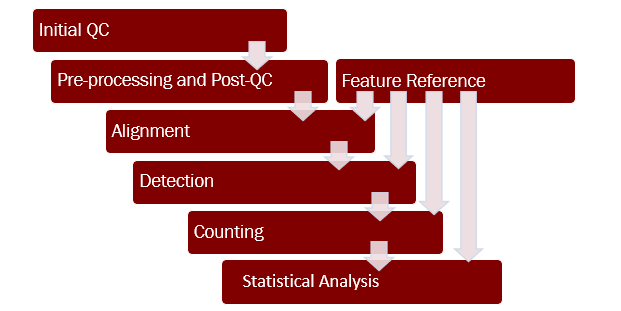
\includegraphics[width = 0.8\textwidth]{figs/ngs-analysis-workflow.png}
\end{figure}

\subsection{Control de calidad inicial}
Los objetivos del control de calidad de las lecturas crudas es detectar problemas de secuenciación, detectar adaptadores y comparar librerías para análisis posteriores. Distintos experimentos requieren interpretaciones distintas del análisis de control de calidad. Una herramienta muy utilizada para esto es FastQC. El análisis de la calidad por base, representa la distribución de las puntuaciones de calidad en todas las lecturas por la posición de cada lectura. En general, es normal que las últimas posiciones tengan una calidad algo peor que las demás, pero una buena muestra debe seguir teniendo una calidad alta. Si una muestra no tiene gran calidad, se puede optar por utilizar solo aquella porción de las muestras que tienen una calidad aceptable, pero hay que tener en cuenta que al acortar las lecturas, el mapeado puede darse en un mayor número de sitios. También se mide el contenido de cada base por posición (que debería ser bastante constante a lo largo de toda la lectura dependiendo de la "complejidad de la muestra", es decir, variedad de tránscritos diferentes) y la puntuación de calidad media por secuencia. La pipeline para el ARNm y los miRNA es la misma, pero hay peculiaridades. Los microARNs son ARNs de unos 20-30 nucleótidos que reprimen la expresión génica de los genes a los que se unen.
Dado el bajo número de miRNAs codificados por el genoma y el más reducido número expresado en cada tejido es de esperar ver perfiles de baja complejidad en las librerías de miRNAs, dádose así un patrón irregular del contenido de bases por posición.

Las secuencias sobrerrepresentadas son listas de secuencias que están presentes más veces de lo esperado por azar. La lista sobrerrepresentada se anota con el tipo de secuencia si se proporciona una lista con la que comparar. Normalmente, las secuencias adaptadoras pueden estar sobrerrepresentadas si hay altos niveles de ligaciones de dímeros de cebadores en el paso de preparación de la biblioteca. A menudo se debe a un desequilibrio entre los niveles de adaptadores y los niveles de fragmentos de muestra. Algunos RNA-Seq de tejidos particulares pueden dar también secuencias sobrerrepresentadas. Por ejemplo, las muestras de sangre contienen grandes cantidades de transcritos de hemoglobina que siempre se reportan como lecturas sobrerrepresentadas. Las muestras de miARN siempre muestran secuencias sobrerrepresentadas. Las bibliotecas de ARN total muestran secuencias sobrerrepresentadas de ARN ribosómicos.

\subsection{Preprocesado}
El preprocesado tiene como objetivo mejorar la calidad, la mapeabilidad, quitar contaminantes y sesgos, etc. Hay diferentes herramientas, como cutadapt o trim-galore. 

La calidad de las bases puede afectar al análisis de llamadas de variantes y, si es grave, también al mapeo de características. La calidad de las bases suele disminuir al final de la lectura y a veces al principio. Además, la secuenciación de baja calidad puede producir un grupo de lecturas de baja calidad a lo largo de su longitud. Es esencial eliminar las bases de baja calidad para el análisis de llamada de variantes. Para otros análisis, elimínelas sólo si afecta al rendimiento del mapeo.

\subsection{Alineamiento y mapeado}
Hay dos tipos de alineamientos: local y global. En el caso del local, se busca que en partes específicas el alineamiento sea bueno, mientras que en el global se busca meter la lectura en la secuencia completa, metiendo gaps. 

La cobertura en un segmento se mide como el número de reads que mapean a ese fragmento del genoma y la longitud de cada lectura dividido por la longitud del fragmento. Para poder hacer el mapeado se necesita la referencia en fasta, las reads en fastq y una referencia indexada. Esto es distinto de los alineadores tradicionales como BLAST. El objetivo es mapear las lecturas a las características. En transcriptómica, el alineamiento se realiza al mismo tiempo que la cuantificación. 

Lo importante es la indexación del genoma de referencia para ahorrar tiempo de computación. El genoma se corta en trozos para que sea más fácil realizar las búsquedas. Esto se puede hacer por ejemplo con BWA y alineadores Bowtie que utilizan la transformación de Burrows-Wheeler al ser más rápidos.

Aunque se hable de expresión génica, los genes no se expresan, son los tránscritos. Con estas técnicas es muy complicado hilar tan fino, por lo que se cuantifican los reads al gen y contar. A la hora de alinear, si se intenta alinear reads al genoma de referencia, las reads salen del tránscrito, por lo que puede ocurrir que una parte de un read caiga en un exón y la otra parte en el otro. Esto se puede visualizar con el visor IGV. Las lecturas partidas se conocen como \textbf{exon junctions}. Por ello, se puede mapear al genoma permitiendo esa característica. Otra opción es alinear directamente al transcriptoma, pero es más grande que el genoma (puede haber 100.000 tránscritos definidos vs 20.000 - 30.000 genes) y puede que haya lecturas que no se puedan mapear a un tránscrito concreto, si no que puedan mapear a varios tránscritos con el mismo exon.

\begin{figure}[h]
\centering
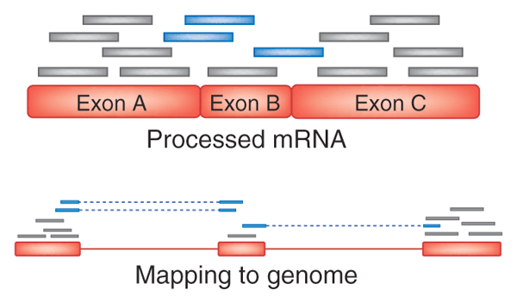
\includegraphics[width = 0.5\textwidth]{figs/Imagen1.png}
\end{figure}

\subsection{Galaxy}
Galaxy es una plataforma con muchas herramientas y workflows ya hechos para investigación biomédica intensiva en datos. Permite generar y hacer públicas pipelines. Se puede utilizar en el servidor europeo o montar un servidor local. 

Para nuestro proyecto, utilizaremos los datos del paper "Next-generation sequencing facilitates quantitative analysis of wild-type and Nrl(-/-) retinal transcriptomes". En la parte de "Related Information" se encuentran los datasets subidos a la base de datos GEO (Gene Expression Omnibus). En general, las revistas buenas exigen poner los datos en una base de datos pública. En este caso hay 6 muestras, 3 wild-type y 3 knock-out. Cada muestra en GEO tiene un ID. 

Galaxy se conecta a las bases de datos mediante API, por lo que se puede poner el link a los reads crudos y Galaxy lo lleva a nuestra sesión sin necesidad de descargarlos de las bases de datos y subirlos a Galaxy de forma manual. 

Nos vamos a descargar la información de los nombres de las muestras (los metadatos). Desde GEO, hay un acceso a SRA Run Selector donde tenemos disponibles esos datos. Hay dos tablas disponibles: metadata y lista de las accesiones con los IDs de las muestras. Los metadatos se necesita posteriormente para saber qué muestras son WT y cuáles KO, pero por ahora solo necesitamos los IDs para subir a Galaxy. El siguiente paso es decirle a Galaxy que, utilizando esos identificadores, se descarguen los FastQ. Para ello, en Get Data hay una opción de Faster Download and Extract Reads in FastQ format from NCBI SRA. Para esa herramienta se selecciona la opción de "List of SRA accessions, one per line" y se ejecuta.

Una vez con los datos, vemos que en Pair-end tenemos 0 datos y en Single-end 6, indicando que las muestras son single-end (aunque esto ya lo sabíamos porque venía en SRA Run Selector). El siguiente paso es ir a FastQC con los datos de single-end. La salida es un fichero txt con los números y un html con las imágenes. Tras analizarlo brevemente, vemos que no hay ningún problema con las muestras, pudiendo continuar con el análisis.

En Ensembl nos vamos a la página de FTP Downloads donde se encuentran todas las referencias de la última versión del genoma. Para reproducir unos resultados, hay que utilizar la referencia de la fecha de publicación de los datos que se estén utilizando, pero en nuestro caso podemos utilizar la última versión generada. Como no queremos descargar el Fasta a nuestro ordenador, vamos al FastA y buscamos el fichero de primary assembly. Con click derecho, podemos copiar el enlace y en Galaxy, en Upload, se puede utilizar la función Paste/Fetch data y pegar ahí la dirección. También subimos el GTF de los cromosomas.

%07/02 - Fátima
El siguiente paso es buscar la herramienta Trim-Galore con los datos single-end dejando todas las opciones como las predeterminadas. Con esta herramienta queremos quitar los adaptadores, y en caso de tener muestras dañadas, podríamos también eliminar esa parte. 

\section{Expresión diferencial}
\subsection{Visualización con IGV}
Para subir un fichero a IGV, nos vamos a File y Load from File. Hay que tener en la misma carpeta el fichero BAM con el fichero BAI, es decir, el fichero indexado. Hay que cargar el BAM. Se muestran tres tracks, siendo uno la cobertura, otro los junctions y el último los duplicados (click derecho y expandir). Previamente hay que seleccionar el genoma correcto; en este caso, el de ratón. 

Podemos irnos al cromosoma 13 y buscar el gen Smn1, con eso saltamos a esa región del genoma. Podemos ver las distintas isoformas del gen y dónde han mapeado las lecturas. En Junctions, vemos que hay lecturas con un arco grande, indicando que la lectura ha mapeado a esos exones que estaban juntos en el tránscrito, pese a que en el genoma estén separados por intrones y otras regiones no codificantes. La cobertura coincide con los exones al tratarse de un RNA-Seq. Además, tiene una cobertura 0-20, indicando que en ese rango hay como máximo 20 reads y como mínimo 0. 

La isoforma superior tiene un exón al principio de la proteína que no tiene ninguna lectura. Esto puede darse por la cobertura baja, indicando que nos estamos perdiendo esa isoforma.

\begin{figure}[h]
\centering
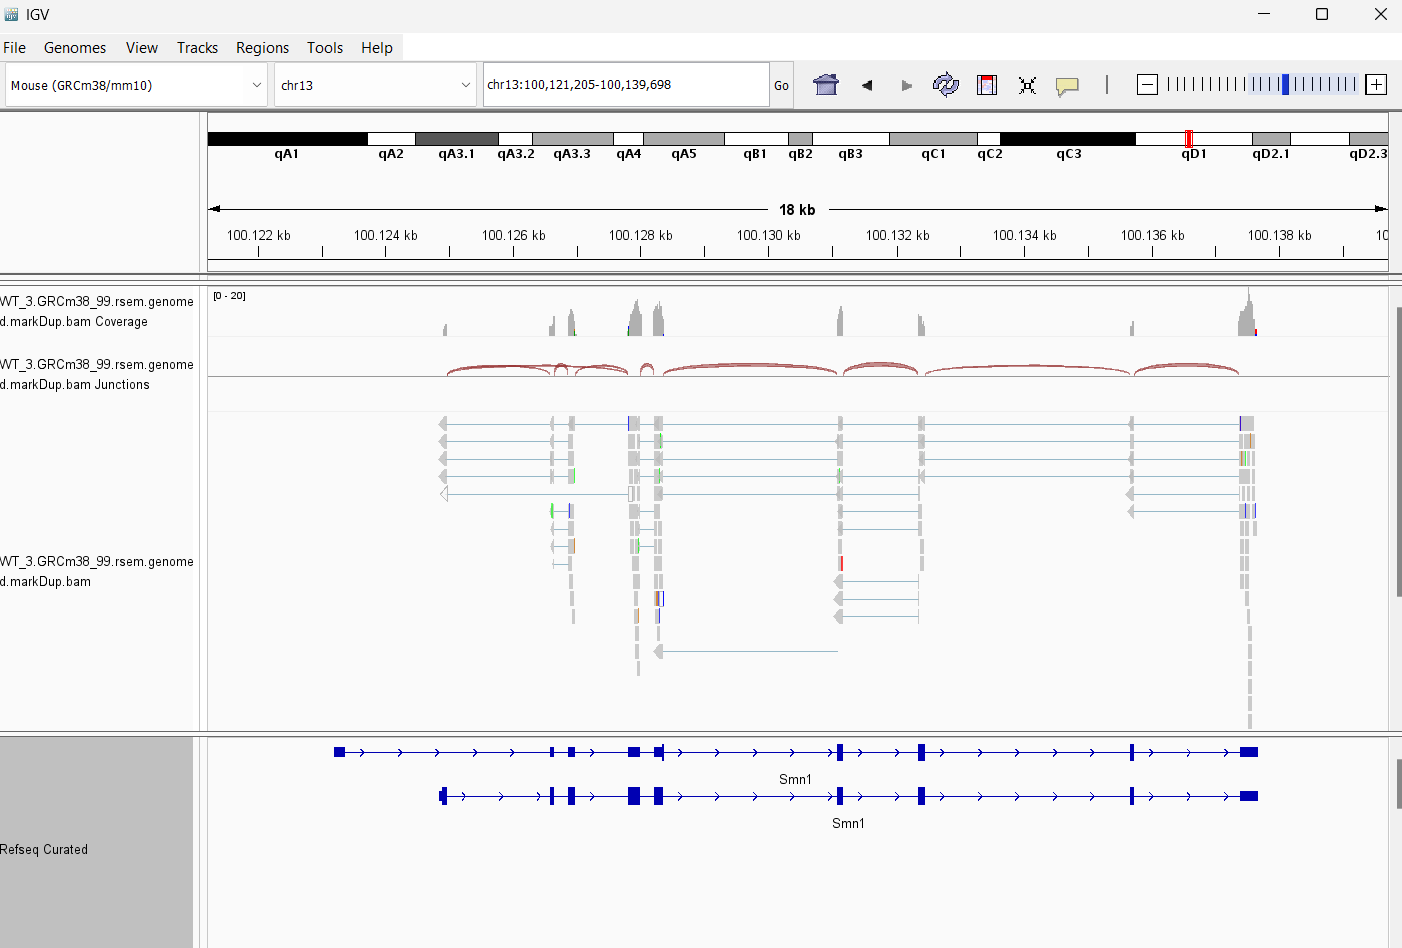
\includegraphics[width = 0.7\textwidth]{figs/igv-1.png}
\end{figure}

\subsection{Redundancia de mapeo}
Pueden darse redundancias de mapeo, ya que la secuencia del genoma es larga y contiene muchas secuencias repetitivas. Por ello, hay que mirar la calidad de mapeado, ya que una lectura puede mapear en un sitio con 1 mismatch y en otra región con 2. Para reducir la ambigüedad en el mapeado (hay genes pareados, isoformas), se puede utilizar pair-end o secuenciación de reads más largas. 

En NGS, se pueden detectar regiones por enriquecimiento viendo, en base a la cobertura del experimento, las regiones donde hay señal y que indicarán genes o factores de transcripción. El proceso es crosslinking, sonicación, inmunoprecipitación y secuenciación. El resultado de este tipo de experimento es un archivo tipo BED o WIG en el que se obtiene la posición donde se encuentra la señal.

En el conteo por ocurrencias, se cuentan cuántas reads caen en las distintas regiones. Para ello se requiere el GTF que asocia los disitntos exones con los tránscritos o isoformas.

En Galaxy, se puede utilizar un solo programa para alinear las lecturas a la referencia y la cuantificación. Al final, no importa si una read pertenece a una isoforma o a otra si queremos abstraer la cuantificación de una proteína, es decir, obtener la cuantificación absoluta. Para la expresión diferencial, se necesita más cobertura y los métodos son un poco diferentes para poder diferenciar las isoformas. Los tránscritos tienen una estructura de dependencia muy complicada, por lo que la expresión diferencial se suele hacer a nivel de gen.

\subsection{Cálculo de expresión}
Una vez con las lecturas mapeando a un gen, si queremos tener una medida robusta de la expresión, hay que tener en cuenta la longitud del gen y el tamaño de la librería. Una librería con una secuenciación mayor, la expresión va a parecer mayor que en una secuenciación con un tamaño menor de librería. Además, un tránscrito más corto va a tener menos reads que caigan en él por mera probabilidad, por lo que hay que normalizar por el tamaño del gen. Para ello, primero se obtienen los counts (la cobertura) y se utilizan los RPKMs:
$$RPKM: 10^9 \cdot \frac{\text{Reads mapped to the transcript}}{\text{Total reads} \cdot \text{Transcript length}}$$
Esta fórmula se modificó a la siguiente para normalizar todo a la vez:
$$TPM = 10^6 \cdot \frac{\text{reads mapped to transcript / transcript length}}{\sum \text{reads mapped to transcript/transcript length}}$$

Para las reads que mapean a varias isoformas o a varios genes del genoma, se utilizan los programas RSEM, Salmon o Sailfish. Estos métodos son procesos iterativos. Se aprovechan de la información de todos los reads para mejorar la probabilidad de qué read pertenece a qué sitio. Teniendo tres isoformas que coinciden en el primer exón, se ven las reads que caen en las partes distintas de los tránscritos para inferir las reads de la parte común de los tránscritos. La probabilidad se va cambiando y ajustando según cambian las probabilidades. Estos métodos probabilísticos hacen una estimación de los counts. Estos algoritmos cuantifican la expresión por isoforma, ya que están hechos para lidiar con el multimapping. La columna IsoPct indica el porcentaje de expresión de esa isoforma sobre toda la expresión del gen completo. Cuando se ve un proceso de splicing alternativo, la isoforma mayoritaria es la primera, y en otra condición puede darse que todas las isoformas estén igual de expresadas o que se convierta en la menos expresada.

El gen SMN1 de ratón es esencial, no puede haber ninguna mutación al ser inviable. De hecho, en humanos, una mutación en este gen causa SMA (spinal muscular atrophy). Esto se debe a que tenemos otro gen, SMN2, que solo se diferencia del 1 en una base y puede ayudar a compensar. Aunque las reads sean prácticamente idénticas, RSEM es capaz de asignarlas a una forma u otra.

\begin{figure}[h]
\centering
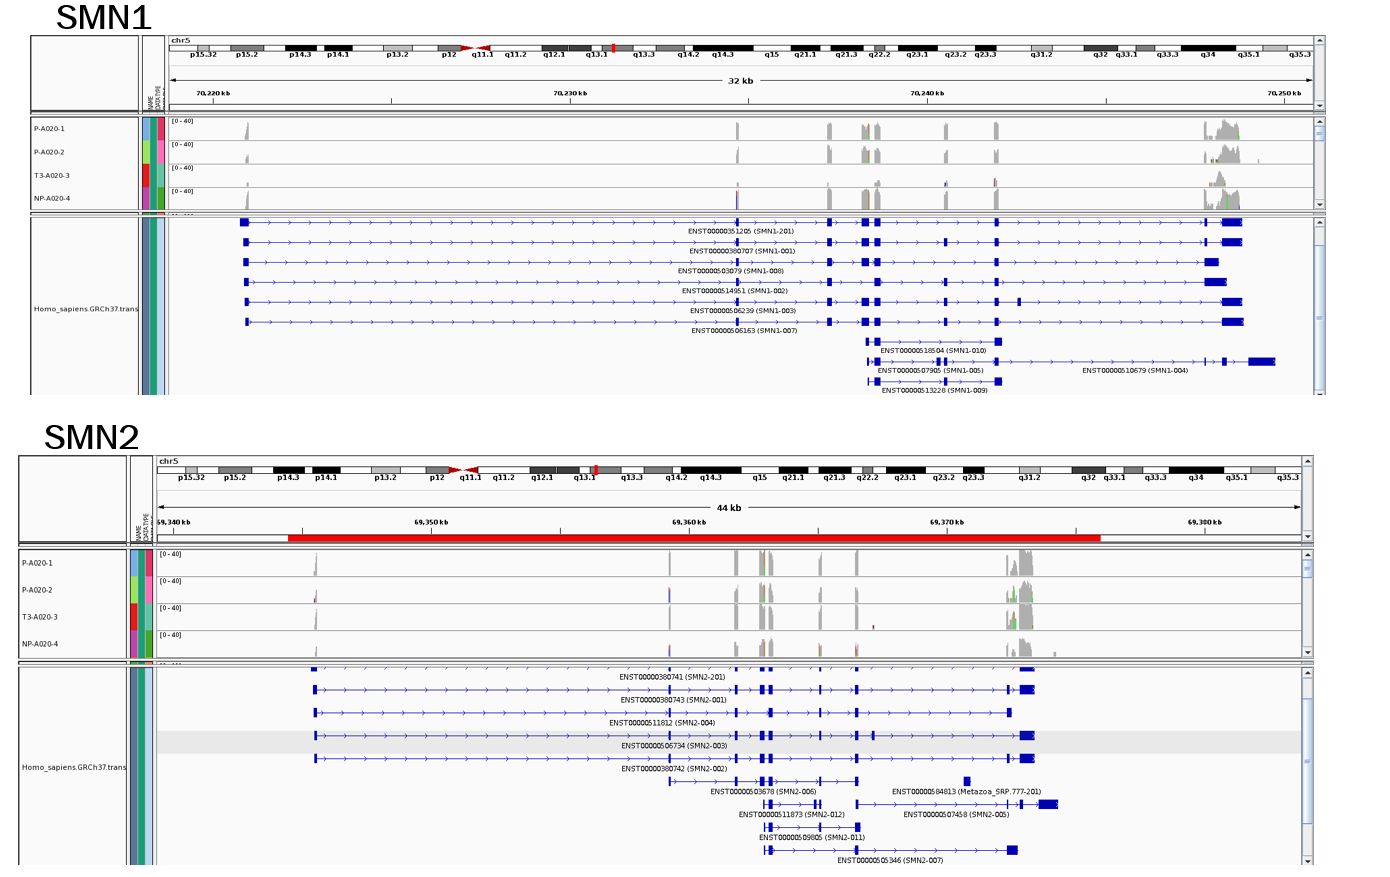
\includegraphics[width = 0.7\textwidth]{figs/smn12.png}
\end{figure}

\subsection{Galaxy}
Volviendo a la práctica, nos vamos a Ensembl y BioMart. Seleccionamos el genoma de ratón, seleccionamos como atributos solo Gene stable ID y transcript stable ID (quitamos los version) y exportamos los resultados como tsv. En Galaxy subimos ese fichero (Gene2Transcript) y utilizamos la herramienta "Sort Column Order by heading" para poner la columna 2 como identificador. 

El siguiente paso es construir la referencia del tránscrito (el fasta del transcriptoma) a partir del GTF que habíamos subido previamente con la herramienta gffread. Debería coger automática el fichero gtf, y en caso contrario lo seleccionamos manualmente. En el apartado de Reference Genome, debemos poner "From your history" para poder indicar el fasta. Además, en "select fasta outputs", seleccionamos la opción de "fasta file with spliced exons for each GFF transcript". También hay que activar "full GFF attribute preservation", y en Feature File Output poner GTF.

%12/02 - Fátima
A continuación utilizamos salmon\_qual utilizando el fichero exons.fa que se acaba de generar.
Los alineadores/mapeadores alinean los reads base a base y cuantifican por exón, tránscrito y gen el número de reads que caen en cada una de esas regiones. Por ello, debe recibir la referencia exons.fa creado a partir del GTF y del Fasta. También recibe la tabla que mapea los tránscritos a los genes (la que hemos construido con el sort column) para conseguir la cuantificación por gen. Aunque nosotros hayamos utilizado salmon, existen otros algoritmos como sailfish y RSEM. En RNA-Seq no quitamos los duplicados al poder significar una mayor expresión. Además, los tres métodos permiten el multimapping para poder ver si las reads van a una u otra isoforma mediante métodos estadísticos de expectation-maximization. 

El resultado contiene el gen (no tránscrito, eso sería otro análisis), la longitud del gen, la longitud efectiva (la que se puede mapear), los TPMs y el número de reads. Esto último es el dato crudo de cuántas reads del experimento caen en ese gen, mientras que los TPMs son los datos normalizados. Para el análisis de expresión diferencial, vamos a utilizar las reads crudas. 

\section{Análisis de expresión diferencial}
\subsection{Galaxy}
Para el análisis de la expresión diferencial, necesitamos una tabla con el ID del gen y las columnas con los reads. Esto lo vamos a hacer dentro de Galaxy con la función cut con el output de salmon y escogiendo las columnas 1 y 5. El siguiente paso es utilizar columnjoin sobre este resultado, siendo la columna 1 el identificador y con 1 línea de encabezado en cada fichero de input.

Con los counts normalizados por el tamaño de gen y de librería, si hiciéramos un plot de expresión sobre lgFC, habría más variabilidad a baja expresión. Limma-voom y trend permite estabilizar la varianza para poder realizar posteriormente el test estadístico. El ejemplo en el que estamos trabajando es bastante sencillo, pero para cuando nos veamos en situaciones más complejas (varias condiciones, medidas repeticas, etc) hay un tutorial de limma escrito por su autor, Gordon Smyth. voom permite meter información sobre la calidad de las réplicas, pero en este caso no vamos a usarlo. Seleccionamos single count matrix. El factor es la variable que determina las condiciones. Por ello, nosotros vamos a añadir un factor llamado genotype y damos para cada muestra el grupo al que pertenece. Esta información está en los metadatos; las primeras tres muestras son WT y las otras tres KO, por lo que debemos proporcionar lo siguiente: WT, WT, WT, KO, KO, KO. 

En Ensembl BioMart, seleccionamos Ensembl Genes y Mouse genes. En Attributes, debemos marcar Gene stable ID y Gene Name y obtener los resultados únicos. Con los resultados descargados, en Galaxy permitimos Gene Annotations y subimos este fichero. Este paso es opcional, es simplemente para que podamos ver mejor los genes. En contrast, debemos poner KO-WT.

A la hora de hacer el análisis de expresión diferencial, cuantas más hipótesis (genes) testemos, más habrá que corregir el p-valor. Por ello, genes no expresados, no aportan información y aumentan el error de tipo 1. Por ello, se pueden quitar los filtrados. En este caso, no queremos quitar aquellos genes que entre las dos condiciones esté downregulado (y en KO no tenga expresión, por ejemplo), pero si un gen no está expresado en más de 4 muestras (de 3 que tenemos por cada condición), sí podemos quitarlos, por lo que sí permitimos el filtrado de genes poco expresados. El filtrado se hace en base de las CPM, poniendo que haya al menos 1 count por million en al menos 3 muestras. Dentro de opciones de salida, seleccionamos todos los posibles plots. 
%esto es lo que pedirá en el ejercicio para que los interpretemos
Del output, siempre hay que usar el p-valor ajustado. 

Por detrás, se ha ejecutado un script de R, que lo veremos más en detalle a continuación. Utilizamos el script \texttt{limma\_example\_rma.r} localizado en la carpeta de prácticas. 

De Galaxy, nos descargamos la tabla resultante (localizada en carpeta de prácticas): Galaxy64-[limma-voom\_KO-WT].tabular. 
Ahora tenemos una colección de genes diferencialmente expresados y tenemos dos opciones: ir mirando uno a uno los genes (por ejemplo, Nlr tiene un p-valor ajustado de $10^{-12}$ y un logFC de -8, es un gen utilizado para el Knock-Out y verificamos que ha funcionado bien. A partir de ahora, buscaríamos rutas de genes que se verían afectados con el KO de este gen. 

Hay dos tipos de análisis funcional: 
\begin{itemize}
\item \textbf{ORA (overrepresentation analysis):} Tenemos 6407 genes diferencialmente expresados de 18387 (obtenidos mediante un filtro de p-valor ajustado < 0.5). Cada uno de los genes se puede clasificar en función del proceso biológico en el que está involucrado (biological process; BP), la función molecular (molecular function; MF) o el compartimento celular (cellular compartment; CC). Para un gen, podemos buscar esto en Gene Ontology Overview. Dentro de cada categoría, hay muchas clases que permiten clasificar los genes de forma cada vez más específica, y un gen puede estar en varias clases. Podemos escoger el número de procesos y la profundidad que deseamos. Asignamos así cada gen a un proceso, y contamos para cada proceso cuántos DEGs hay. Este número se compara con los valores de Whole genome. Aquellas proporciones muy enriquecidas son las que se marcan como cambio significativo. Así, se puede decir que el experimento afecta sobre todo al proceso x (por ejemplo, regulación génica). En caso de no obtener ningún DEG, se podrían utilizar filtros más laxos, o utilizar GSEA. 
\item \textbf{GSEA (gene set enrichment analysis):} para este método, se cogen la lista de todos los genes y se ordenan de menor a mayor en función de su logFC (aunque se puede elegir en función de qué hacer la ordenación). Seguimos teniendo la lista con los procesos a los que pertenecen los genes. Por ello, podemos ver dónde caen los genes de cada proceso. Si para un proceso todos los genes se encuentran cerca, esto se puede reportar (tienen una magnitud de cambio similar; el experimento perturba ese proceso). 
\end{itemize}
 
En el NIH está la herramienta \href{https://davidbioinformatics.nih.gov/}{DAVID} que permite subir una lista o un background (pestaña functional annotation). En el caso de los arrays, no se miran todos los genes, por lo que no tiene sentido comparar en el ORA con whole genome, si no que se utiliza otro background (por ejemplo, solo el cromosoma 1, lo que se utilice como total). En nuestro caso copiamos los primeros 150 gene ID, pero también se podría subir en forma de fichero. Se selecciona que los identificadores sean de genes de Ensembl y que se trata de una lista, no background. Hay 14 genes que no se pueden detectar con esta herramienta, pero es algo asumible. Aparece una pestaña de Gene Ontology que especifica los distintos niveles de las tres partes (BP, MF y CC). Por ejemplo, para BP, hay 5 niveles, cada uno a un mayor nivel. En direct, se mezclan los distintos niveles para obtener una clasificación que sea detallada, pero sin ser exhaustiva. Como se están testando muchos genes, hay que volver a hacer el ajuste del p-valor, que en este caso aparece en una columna con la corrección de Benjamini. Esto sería el equivalente al ORA.
%Importante describir bien esta parte.

%14/02 - Carlos Torroja
\chapter{ChIP-Seq}
\section{Procedimiento experimental}
ChIP-Seq (Chromatin Immunoprecipitation Sequencing) es una técnica diseñada para identificar las regiones del ADN donde se unen los factores de transcripción. Utiliza secuenciación de nueva generación (NGS) de lecturas cortas (short reads) y se basa en la inmunoprecipitación de factores de transcripción. Si no se dispone de un anticuerpo específico para el factor de transcripción de interés, la técnica no puede llevarse a cabo.

El procedimiento experimental es el siguiente:
\begin{enumerate}
\item \textbf{Fijación y fragmentación del ADN:} Se fijan las células de un tejido con un agente químico para mantener el factor de transcripción unido al ADN. Se extrae el ADN junto con las proteínas unidas y se fragmenta mediante sonicación, obteniendo fragmentos de aproximadamente 200 pares de bases, ideal para la secuenciación con tecnología Illumina. Este tamaño permite además acotar la región donde buscar posteriormente los enriquecimientos.
\item \textbf{Inmunoprecipitación:} Se introduce un anticuerpo específico para el factor de transcripción en la solución de fragmentos de ADN.
Como control, se puede preparar una muestra sin anticuerpo para evaluar la distribución del coverage del genoma.
Los fragmentos de ADN unidos al factor de transcripción se capturan utilizando una columna con bolitas que se unen a la región constante del anticuerpo.
\item \textbf{Preparación de la librería y secuenciación:} Se deshace la fijación para eliminar las proteínas y se prepara la librería de ADN para secuenciar.
Se realiza la secuenciación, idealmente obteniendo entre 20 y 40 millones de lecturas (reads).
\end{enumerate}

\section{Análisis de Datos}
\paragraph{Alineamiento de lecturas}
Las lecturas se alinean al genoma de referencia. En general, se utiliza secuenciación single-end, donde las lecturas no están pareadas.
Se observa un patrón donde las lecturas se alinean en la región 5' en un sentido y en la región 3' en sentido inverso, lo que indica la señal de enriquecimiento.

\paragraph{Identificación de regiones enriquecidas}
Se utilizan herramientas como MACS (Model-based Analysis of ChIP-Seq) para identificar regiones enriquecidas.
MACS modela una distribución nula, fragmenta el genoma en bins y calcula el número de lecturas en cada bin.
La herramienta desplaza y junta los picos de las distribuciones (una por cada sentido) para aumentar la señal y evaluar las regiones enriquecidas en comparación con el control.

\paragraph{Análisis de motivos de unión}
Se identifican las secuencias de ADN donde se une el factor de transcripción y los genes asociados.
Se utilizan herramientas para buscar motivos enriquecidos de 10-15 nucleótidos mediante el algoritmo de expectation-maximization.
Esto permite estimar la secuencia consenso de unión y predecir otros sitios potenciales en el genoma mediante el logo generado.

\section{Aplicación práctica: Pipeline de análisis con Galaxy}
Vamos a construir una pipeline para analizar datos de ChIP-Seq del artículo \href{https://www.sciencedirect.com/science/article/pii/S2211124713001368?via\%3Dihub}{"Analysis of the DNA-binding profile and function of tale homeoproteins reveals their specialization and specific interactions with hox genes/proteins"}. Este estudio evalúa los sitios de unión de tres factores de transcripción: Prep1, Meis1 y Pbx1, relacionados con los genes Hox del desarrollo embrionario.


%%% Apuntes en crudo 

Se realizan tres ChIP-Seqs con tres anticuerpos (uno para cada factor). Meis1 salió muy ruidoso, prep1 tenía unos picos muy marcados, y pbx1 algo itnermedio. Los picos de meis tenían dos distribuciones, y donde estaba prep meis también tenía un pico marcado. 

El Galaxy (el americano), vamos a Histories > Public Histories > cartof e importamos la historia "Pbx1 ChIPSeq Raw Data". En Pubmed, buscamos el paper en cuestión y en additional information tenemos el enlace a GEO. De ahí podemos ir a SRA Run Selector, donde podemos ver las tablas con todas las muestras del artículo. Hay dos tipos de Assay Type: RNA-Seq y ChIP-Seq, y a nosotros nos interesa el último. Los tamaños de ficheros son grandes (3 Gb), e importarlos a Galaxy tarda un poco. Lo que podemos hacer es seleccionar las muestras y darle al botón de arriba de "Computing Galaxy". Esto sirve para el Galaxy americano; para el europeo tendríamos que bajarnos las tablas de metadatos. 

Para la pipeline, suponemos que partimos de esto, la tabla de SRA subida en Galaxy. Desde ahí vamos creando todo el procesamiento. Las anotaciones de los campos son muy libres y no hay estándar, por lo que la pipeline se debe adaptar al contenido de los datos concretos. Primero debemos quedarnos con las columnas que nos interesan: run (columna 1), library name (columna 17) y chip\_antibody (columna 32). Con esto nos vamos a cut columns y lo ejecutamos. Al analizar el contenido, vemos que algunas celdas contienen dos puntos, espacios, paréntesis... cosas que para herramientas bioinformáticas puede ser perjudicial. Por ello utilizamos la herramienta column regex find and replace. Seleccionamos la columna 2 y utilizamos una expresión regular: \texttt{.*WT\symbol{92}s([\symbol{92}w\symbol{92}s]+)} y se reemplaza por \symbol{92}1. Además, queremos sustituir los espacios por una barra baja. Para esto, creamos un segundo check que trabaje sobre el output del anterior (find regex \symbol{92}s replace \_.

Mientras tanto, vamos modificando la columna 3. Utilizamos la misma herramienta: regex [\symbol{92}/\symbol{92}s].+ replace por nada (se deja el campo en blanco). Este va a ser el input para empezar el workflow. En el workflow, no hay una referencia, por lo que es necesario un paso de detección de los picos. Esto sería lo que haría MACS, junto con el contaje y el análisis estadístico.

Ahora utilizamos la herramienta Faster Download and Extract Reads in FastQ format. A partir de esa tabla, construimos una lista de SRR para utilizar esta herramienta. En la pestaña de Workflows, creamos uno nuevo. El workflow permite incluir casillas de "input" que al generar el workflow se convierten en casillas que hay que rellenar a mano. Vamos a incluir un input dataset y ponemos como label SRA Table. En la anotación podemos incluir los requerimientos mínimos "Sample table with SRR column and sample name column." y ponemos como format "tabular". El siguiente paso ponemos la herramienta cut con nombre "extract SRR column". En los parámetros de la herramienta, se pueden "desactivar", de forma que al ejecutar el workflow pida el input. Otra opción es pulsar a las dos flechas e incluir un input de texto donde ponemos "SRR Column". Ese input podemos linquearlo al input de cut columns. También hay que eliminar la primera fila que incluye la cabecera del fichero y que no queremos incluir como SRR mediante la herramienta "select last lines from a database (tail)". Esta herramienta permite elegir "keep everything from this line on" y la segunda fila, de forma que no importe cómo de grande es el dataset. Como todo esto son pasos intermedios, podemos tachar el símbolo del ojo para que no aparezca en la historia y no cause ruido visual. A continuación podemos incluir la herramienta de descarga. A priori no tiene input, pero podemos seleccionar la opción "list of SRA accession, one per line" e incluir el input. Esta herramienta saca cuatro outputs. Si la secuenciación es single-en, el output importante es "output\_collection", mientras que si es paired-end, es "list\_paired". No se puede seleccionar un solo tipo de entrada, solo podemos escoger la salida que nos interese.

Tras ejecutar esto, se realiza el FastQC, Trim-Galore para eliminar los adaptadores de la secuencia y aumentar la capacidad de alinear, alinear para saber la parte del genoma de donde provienen las reads. En este caso, utilizaremos BWA. Le debemos dar una referencia (genoma de ratón). En el fastqc se puede ver que las regiones son de 35 nucleótidos, por lo que no se buscan gaps ni otros eventos, pudiendo utilizar la herramienta bwa estándar. 

Tras alinear, tenemos el fichero BAM. Se hace un control de calidad para ChIP-Seq con la herramienta plotFingerprint, el cual fragmenta el genoma en pequeños fragmentos y va contando las reads que hay en cada fragmento. Esto se hace para todas las muestras. Luego genera un plot con esa información en el que vienen los fragmentos por counts y se hace un plot cumulativo. 

La detección se realiza en base a un patrón o en base al enriquecimiento. Para definir un tránscrito, debe estar enriquecido y cumplir con un patrón. EN el caso de los picos, la detección es simplemente "enrichment-based". El transcriptoma debe ser compatible con las características que queremos detectar (miRNA, mRNA, sitio de unión a factor de transcripción). 

MACS2 busca las dos distribuciones, mira la distancia entre los picos de ambas y busca distribuciones opuestas en un rango pequeño (rango de la sonicación, unos 200 pares de bases). Ese parámetro se incorpora a la herramienta. Junta las dos distribuciones en un pico central para aumentar la detección. Luego hace búsquedas en distintos tamaños de fragmento ys e queda con el que mejor se adapta. Así, simula la distribución nula con los datos. 
En la herramienta MACS2 hay que añadir algunos parámetros: el tamaño efectivo del genoma de referencia, incluir peak summits de los outputs adicionales. Con este archivo bed se ordena por el score de mayor a menor y se buscan los motivos de unión del factor de transcripción. Para buscar la secuencia, se cogen las zonas donde se une y se busca el patrón con la herramienta MEME. MEME parte de secuencias, pero partimos de un nucleótido. EN los siguientes pasos aumentamos el número en 50 nucleótidos en ambas direcciones. Esta colección de regiones se puede filtrar para quedarnos con los 500 más altos y con la herramienta Extract Genomic DNA saca la secuencia que define la región de cada fila del bed. Esto se mete en MEME y obtenemos los logos. Con la flecha en Submit/Download podemos buscar ese logo en la base de datos para buscar otras secuencias iguales recogidas. 